\documentclass{article}
\usepackage[letterpaper, total={6in, 8in}]{geometry}
\usepackage[smartEllipses]{markdown}
\usepackage[utf8]{inputenc}
\usepackage{natbib}
\usepackage{graphicx}
\usepackage{enumitem}
\usepackage{hyperref}
\usepackage{float}
\usepackage[table,xcdraw]{xcolor}
\usepackage{bookmark}
\usepackage{listings}
\usepackage{algpseudocode}
\usepackage{algorithm}

\title{CS 2300 Database Project \\ Phase III}
\author{Jack Kufa}
\date{\today}

\begin{document}
\maketitle

\section*{Problem Statement}
I build a Discord bot and localhost web application for managing and automating a Pokemon Draft League. A Pokemon Draft League is a custom game mode
for Pokemon battling, where coaches form teams and draft Pokemon to compete head to head. This application is able to automate 
a lot of the internal work involved in running such a league and it streamlines specific aspects of league upkeep such as updating rankings.

The core interface is the Discord Bot. 
This is because Discord is a vital platform for communication between players, and being able to query data in that same space is very convenient. 
With that said, the web application, built for administrative use, is perfect to getting a league up and running.

\section*{ER Model}
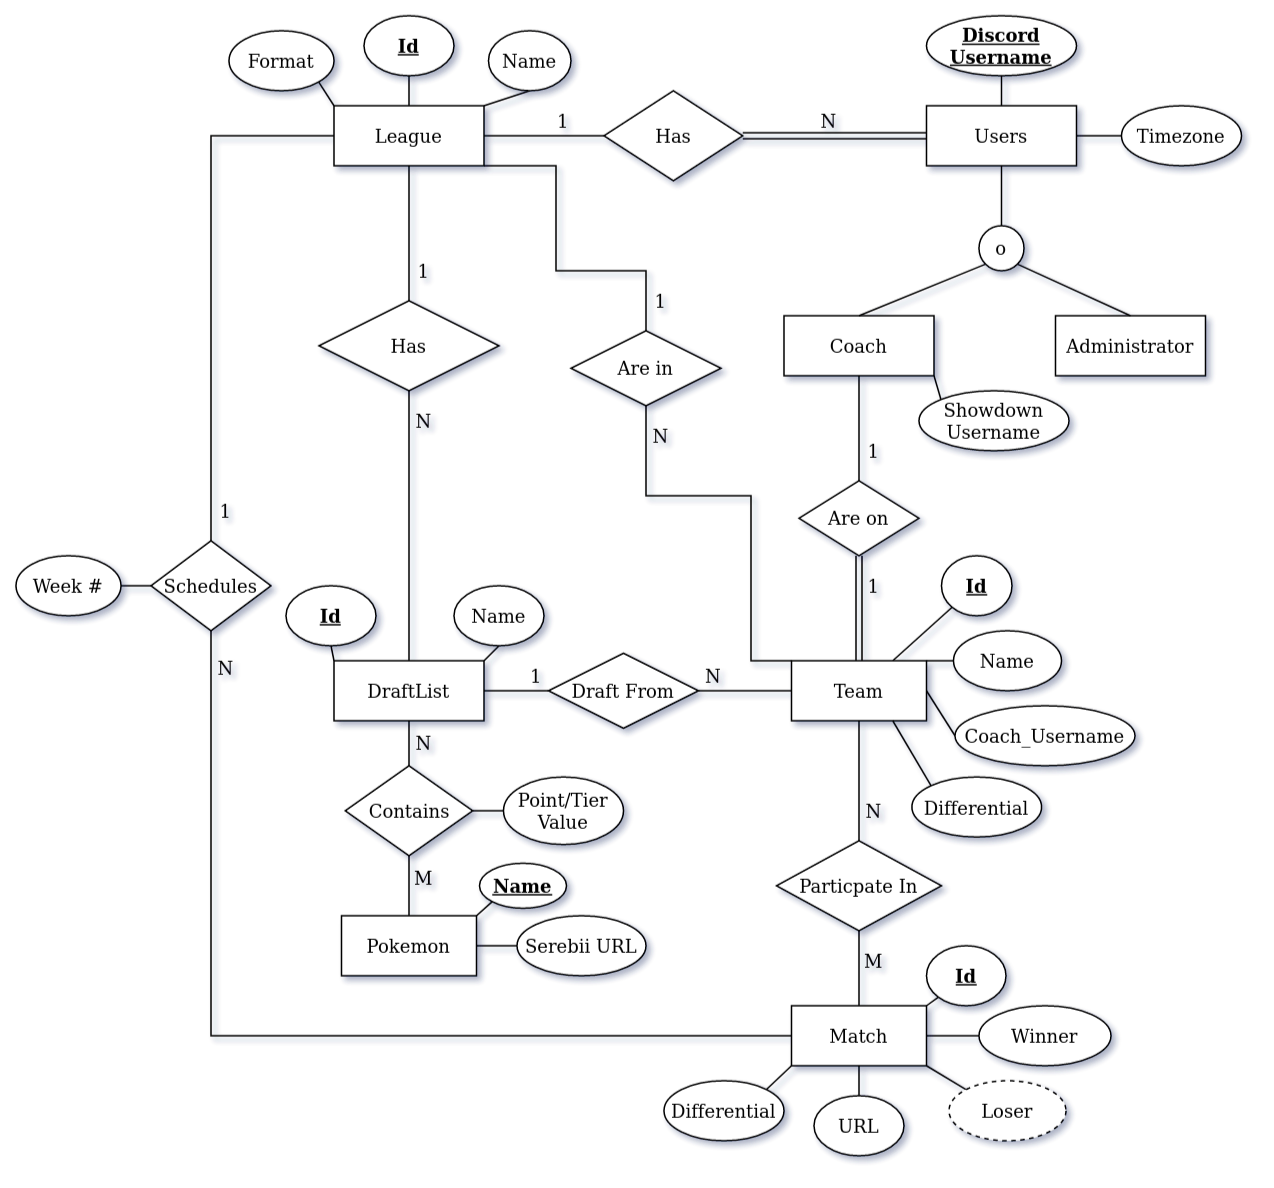
\includegraphics[scale=.35]{PokemonDraftLeagueDB_final.png}

The six primary entity sets are as follows:
\begin{enumerate}
    \item League: The Main entity that specifies the battle format and draft list being used. Essentially every other entity is related to the league in some capacity.
    \item Users: Users who are participating in the league. The subclasses are as follows: \begin{enumerate}
        \item Coach: Think of it like the coach of a sports team. These are the players that are actually participating in the league.
        \item Administrator: A person who has additional privileges for managing the league.
        \item[*] It should be noted that a user can be either a coach or an administrator, or both, but it cannot be neither.
    \end{enumerate}
    \item Teams: Another big entity which is essentially an equivalent of a sports team. It has a team name, coach username, and differential. 
    The differential is an integer value that equates to the total number of Pokemon beaten in any match.
    \item Pokemon: This entity is used to represent the creatures used in battle; think of them as the players for a sports team. 
    Each Pokemon has a name, and for convenience of the user, a url to the \href{https://www.serebii.net/}{Serebii} page, which has important information such as Pokemon Type, move set, and stats. 
    A draft list contains Pokemon, associated each with a point value.
    \item DraftList: This is the reference sheet used for drafting Pokemon. Each Pokemon in a draft list has an associated value that indicates its "cost" in the draft league, including a list of banned Pokemon.
    \item Match: This entity is for storing information related to Pokemon battles. Matches are played on \href{https://pokemonshowdown.com/}{Pokemon Showdown}. 
    This entity stores the match's url, differential (The difference in knocked out Pokemon on either side), and winner, meaning that  subsequently a loser can also be derived.
\end{enumerate}
There are some aspects of this entity relationship diagram that should be noted. 
First, any tables that potentially would have contained multivalued attributes, such as a team's Pokemon, were optimized to 1NF specifications so that no multivalued attributes were actually needed. 
Second, there is a redundant relationship that exists, the relationship between the league and teams. 
This relationship was added due to time constraints, for there were times where querying a team based on its league proved to be infinitely more convenient than querying users first. Ideally, however, this is a relationship that is unnecessary.
\section*{Logical Database Design}
% \includegraphics[scale=.38]{Logical_DB_final.png}\newpage
\section*{Summary of Data Types}
\begin{table}[H]
    \large
    \centering
    \begin{tabular}{|l|l|l|l|}
    \hline
    {\color[HTML]{2E3436} \textbf{Table}} & {\color[HTML]{2E3436} \textbf{Attribute}} & {\color[HTML]{2E3436} \textbf{Type}} & {\color[HTML]{2E3436} \textbf{Constraint}} \\ \hline
    {\color[HTML]{2E3436} League} & {\color[HTML]{2E3436} Id} & {\color[HTML]{2E3436} INTEGER} & {\color[HTML]{2E3436} Primary Key} \\ \hline
    {\color[HTML]{2E3436} League} & {\color[HTML]{2E3436} Name} & {\color[HTML]{2E3436} VARCHAR(256)} & {\color[HTML]{2E3436} Unique} \\ \hline
    {\color[HTML]{2E3436} League} & {\color[HTML]{2E3436} Format} & {\color[HTML]{2E3436} VARCHAR(20)} & {\color[HTML]{2E3436} } \\ \hline
    {\color[HTML]{2E3436} League} & {\color[HTML]{2E3436} Dlist\_id} & {\color[HTML]{2E3436} INTEGER} & {\color[HTML]{2E3436} Foreign Key} \\ \hline
    {\color[HTML]{2E3436} User} & {\color[HTML]{2E3436} Username} & {\color[HTML]{2E3436} VARCHAR} & {\color[HTML]{2E3436} Primary Key} \\ \hline
    {\color[HTML]{2E3436} User} & {\color[HTML]{2E3436} Timezone} & {\color[HTML]{2E3436} CHAR(6)} & {\color[HTML]{2E3436} } \\ \hline
    {\color[HTML]{2E3436} User} & {\color[HTML]{2E3436} League\_id} & {\color[HTML]{2E3436} INTEGER} & {\color[HTML]{2E3436} Foreign Key} \\ \hline
    {\color[HTML]{2E3436} Coach} & {\color[HTML]{2E3436} Discord\_username} & {\color[HTML]{2E3436} VARCHAR} & {\color[HTML]{2E3436} Foreign Key} \\ \hline
    {\color[HTML]{2E3436} Coach} & {\color[HTML]{2E3436} Showdown\_username} & {\color[HTML]{2E3436} VARCHAR} & {\color[HTML]{2E3436} Unique} \\ \hline
    {\color[HTML]{2E3436} Administrator} & {\color[HTML]{2E3436} Discord\_Username} & {\color[HTML]{2E3436} VARCHAR} & {\color[HTML]{2E3436} Foreign Key} \\ \hline
    {\color[HTML]{2E3436} Team} & {\color[HTML]{2E3436} Id} & {\color[HTML]{2E3436} INTEGER} & {\color[HTML]{2E3436} Primary Key} \\ \hline
    {\color[HTML]{2E3436} Team} & {\color[HTML]{2E3436} League\_id} & {\color[HTML]{2E3436} INTEGER} & {\color[HTML]{2E3436} } \\ \hline
    {\color[HTML]{2E3436} Team} & {\color[HTML]{2E3436} Name} & {\color[HTML]{2E3436} VARCHAR(80)} & {\color[HTML]{2E3436} Unique} \\ \hline
    {\color[HTML]{2E3436} Team} & {\color[HTML]{2E3436} Differential} & {\color[HTML]{2E3436} INTEGER} & {\color[HTML]{2E3436} } \\ \hline
    {\color[HTML]{2E3436} Team} & {\color[HTML]{2E3436} Coach\_username} & {\color[HTML]{2E3436} VARCHAR} & {\color[HTML]{2E3436} Foreign Key} \\ \hline
    {\color[HTML]{2E3436} DraftList} & {\color[HTML]{2E3436} Id} & {\color[HTML]{2E3436} INTEGER} & {\color[HTML]{2E3436} Primary Key} \\ \hline
    {\color[HTML]{2E3436} DraftList} & {\color[HTML]{2E3436} Name} & {\color[HTML]{2E3436} VARCHAR(50)} & {\color[HTML]{2E3436} Unique} \\ \hline
    {\color[HTML]{2E3436} Pokemon} & {\color[HTML]{2E3436} Name} & {\color[HTML]{2E3436} VARCHAR(25)} & {\color[HTML]{2E3436} Primary Key} \\ \hline
    {\color[HTML]{2E3436} Pokemon} & {\color[HTML]{2E3436} Url} & {\color[HTML]{2E3436} VARCHAR(60)} & {\color[HTML]{2E3436} } \\ \hline
    {\color[HTML]{2E3436} Match} & {\color[HTML]{2E3436} Id} & {\color[HTML]{2E3436} INTEGER} & {\color[HTML]{2E3436} Primary Key} \\ \hline
    {\color[HTML]{2E3436} Match} & {\color[HTML]{2E3436} Week\_no} & {\color[HTML]{2E3436} INTEGER} & {\color[HTML]{2E3436} } \\ \hline
    {\color[HTML]{2E3436} Match} & {\color[HTML]{2E3436} Differential} & {\color[HTML]{2E3436} INTEGER} & {\color[HTML]{2E3436} } \\ \hline
    {\color[HTML]{2E3436} Match} & {\color[HTML]{2E3436} Url} & {\color[HTML]{2E3436} VARCHAR(60)} & {\color[HTML]{2E3436} } \\ \hline
    {\color[HTML]{2E3436} Match} & {\color[HTML]{2E3436} Winner} & {\color[HTML]{2E3436} VARCHAR(80)} & {\color[HTML]{2E3436} } \\ \hline
    {\color[HTML]{2E3436} Match\_League} & {\color[HTML]{2E3436} league\_id} & {\color[HTML]{2E3436} INTEGER} & {\color[HTML]{2E3436} Primary Key, Foreign Key} \\ \hline
    {\color[HTML]{2E3436} Match\_League} & {\color[HTML]{2E3436} Match\_id} & {\color[HTML]{2E3436} INTEGER} & {\color[HTML]{2E3436} Primary Key, Foreign Key} \\ \hline
    {\color[HTML]{2E3436} DraftList\_Pokemon} & {\color[HTML]{2E3436} Pkmn\_name} & {\color[HTML]{2E3436} VARCHAR(25)} & {\color[HTML]{2E3436} Primary Key, Foreign Key} \\ \hline
    {\color[HTML]{2E3436} DraftList\_Pokemon} & {\color[HTML]{2E3436} Dlist\_id} & {\color[HTML]{2E3436} INTEGER} & {\color[HTML]{2E3436} Primary Key, Foreign Key} \\ \hline
    {\color[HTML]{2E3436} DraftList\_Pokemon} & {\color[HTML]{2E3436} Value} & {\color[HTML]{2E3436} VARCHAR(10)} & {\color[HTML]{2E3436} } \\ \hline
    {\color[HTML]{2E3436} Pokemon\_Team} & {\color[HTML]{2E3436} Pkmn\_name} & {\color[HTML]{2E3436} VARCHAR(25)} & {\color[HTML]{2E3436} Primary Key, Foreign Key} \\ \hline
    {\color[HTML]{2E3436} Pokemon\_Team} & {\color[HTML]{2E3436} Team\_id} & {\color[HTML]{2E3436} INTEGER} & {\color[HTML]{2E3436} Primary Key, Foreign Key} \\ \hline
    {\color[HTML]{2E3436} Team\_Match} & {\color[HTML]{2E3436} Team\_id} & {\color[HTML]{2E3436} INTEGER} & {\color[HTML]{2E3436} Primary Key, Foreign Key} \\ \hline
    {\color[HTML]{2E3436} Team\_Match} & {\color[HTML]{2E3436} Match\_id} & {\color[HTML]{2E3436} INTEGER} & {\color[HTML]{2E3436} Primary Key, Foreign Key} \\ \hline
    \end{tabular}
\end{table}
\section*{Application Program Design (Functionality)}
The following is psuedocode for some of the functions that have been implemented. 
Please note that while the query syntax is made to mimic SQL, it is not 100\% the same syntactically, and should not be treated as such.
\begin{itemize}
    \item \textsc{Basic Functions:}
    \begin{enumerate}
        \item Draft Pokemon (Insert): 
        \begin{algorithm}[H]
            \verb|!draft <Pokemon Name>|
            \label{pseudoPSO}
            \begin{algorithmic}
                \Function {Draft\_Pokemon}{$discord\_username$, $user\_message$}
                \If{POKEMON \textbf{contains} $user\_message$}
                \State{$pokemon$ = \textbf{SELECT} $Name$ \textbf{FROM} POKEMON}
                \State{\quad\quad\quad\quad\quad \textbf{WHERE} $Name=user\_message$}
                \State{$coach$ = \textbf{SELECT} $Name$ \textbf{FROM} COACH}
                \State{\quad\quad\quad\quad\textbf{WHERE} $Name=discord\_username$}
                \State{\textbf{INSERT INTO} POKEMON\_TEAM $Pokemon\_Name$, $Team\_Name$}
                \State{\textbf{VALUES} $pokemon$, $coach$}
                \State{\textbf{print} "You selected: " + $pokemon$}
                \Else{ \textbf{print } "ERROR. That is not a valid Pokemon!"}
                \EndIf
                \EndFunction
            \end{algorithmic}
        \end{algorithm}
        \item Submit Replay (Insert): 
        \begin{algorithm}[H]
            \verb|!submit <Replay URL>|
            \label{pseudoPSO}
            \begin{algorithmic}
                \Function {Submit\_Replay}{$user\_message$}
                \If{$user\_message$ \textbf{starts with} https://replay...}
                \State{Parse website data for $winner$, $loser$, $differential$, and $id$}
                \State{\textbf{INSERT INTO} MATCH $ID$, $Differential$}
                \State{\textbf{VALUES} $id$, $differential$}
                \State{\textbf{INSERT INTO} MATCH\_PLAYERS $Winner$, $Loser$}
                \State{\textbf{VALUES} $winner$, $loser$}
                \EndIf
                \EndFunction
            \end{algorithmic}
        \end{algorithm}
        \item Redraft Pokemon (Modify):
        \begin{algorithm}[H]
            \verb|!redraft <Pokemon Name 1> <Pokemon Name 2>|
            \label{pseudoPSO}
            \begin{algorithmic}
                \Function {Redraft\_Pokemon}{$discord\_username$, $user\_message$ [ ]}
                \State{\textbf{Split} $user\_message$ \textbf{into} $find$ \textbf{and} $replace$}
                \If{POKEMON \textbf{contains} $replace$}
                \State{$find\_pokemon$ = \textbf{SELECT} $Name$ \textbf{FROM} POKEMON}
                \State{\quad\quad\quad\quad\quad\quad\quad\quad \textbf{WHERE} $Name=find$}
                \State{$replace\_pokemon$ = \textbf{SELECT} $Name$ \textbf{FROM} POKEMON}
                \State{\quad\quad\quad\quad\quad\quad\quad\quad\quad\textbf{WHERE} $Name=replace$}
                \State{\textbf{UPDATE } $POKEMON\_COACH$}
                \State{\textbf{SET } $Pokemon\_Name=replace$}
                \State{\textbf{WHERE }$Pokemon\_Name=find$}
                \State{\textbf{print } $find$ + " Has been replaced with " + $replace$}
                \Else{\textbf{ print } "ERROR. That is not a valid Pokemon!"}
                \EndIf
                \EndFunction
            \end{algorithmic}
        \end{algorithm}
        \item Delete User (Remove):
        \begin{algorithm}[H]
            \verb|!delete <username>|
            \label{pseudoPSO}
            \begin{algorithmic}
                \Function {Delete\_User}{$user\_message$}
                \State{\textbf{Split} $user\_message$ \textbf{into} $find$ \textbf{and} $replace$}
                \If{POKEMON \textbf{contains} $replace$}
                \State{$find\_pokemon$ = \textbf{SELECT} $Name$ \textbf{FROM} POKEMON}
                \State{\quad\quad\quad\quad\quad\quad\quad\quad \textbf{WHERE} $Name=find$}
                \State{$replace\_pokemon$ = \textbf{SELECT} $Name$ \textbf{FROM} POKEMON}
                \State{\quad\quad\quad\quad\quad\quad\quad\quad\quad\textbf{WHERE} $Name=replace$}
                \State{\textbf{UPDATE } $POKEMON\_COACH$}
                \State{\textbf{SET } $Pokemon\_Name=replace$}
                \State{\textbf{WHERE }$Pokemon\_Name=find$}
                \State{\textbf{print } $find$ + " Has been replaced with " + $replace$}
                \Else{\textbf{ print } "ERROR. That is not a valid Pokemon!"}
                \EndIf
                \EndFunction
            \end{algorithmic}
        \end{algorithm}
    \end{enumerate}
    \begin{enumerate}
        \item Query all of a user's info (join):
        \begin{algorithm}[H]
            \verb|!userinfo <User>|
            \label{pseudoPSO}
            \begin{algorithmic}
                \Function {User\_Info}{$user\_message$}
                \If{USER \textbf{contains} $user\_message$}
                \State{R$1$ = \textbf{INNER JOIN} USER$.Discord\_Username$ = COACH$.Discord\_Username$}
                \State{$R2$ = \textbf{INNER JOIN} R1$.Discord\_Username$ = COACH\_TEAM$.Coach\_Username$}
                \State{$info$ = \textbf{SELECT} $Discord\_Username, Team\_Name, Showdown\_Name$ \textbf{FROM} $R2$}
                \State{\qquad\quad \textbf{ WHERE }$Discord\_Name=user\_message$}
                \State {\textbf{print } $info$}
                \EndIf
                \EndFunction
            \end{algorithmic}
        \end{algorithm}
        \item Calc Average Differential (Join,Average):
        \begin{algorithm}[H]
            \verb|internal function|
            \label{pseudoPSO}
            \begin{algorithmic}
                \Function {Differential}{$team\_name$}
                \State{$positive$ = \textbf{SELECT SUM} $Differential$ \textbf{FROM} MATCH}
                \State{\qquad\qquad\quad \textbf{WHERE} MATCH.$Winner=team\_name$}
                \State{$negative$ = \textbf{SELECT SUM} $Differential$ \textbf{FROM} MATCH}
                \State{\qquad\qquad\quad \textbf{WHERE} MATCH.$Loser=team\_name$}
                \State{\textbf{SELECT AVG} $Differential$ \textbf{FROM} MATCH}
                \State{\textbf{return} $positve-negative$}
                \EndFunction
            \end{algorithmic}
        \end{algorithm}
        \item Query rankings (Order By):
        \begin{algorithm}[H]
            \verb|!rankings|
            \label{pseudoPSO}
            \begin{algorithmic}
                \Function {Rankings}{}
                \State{$rankings$ = \textbf{SELECT} $team$ \textbf{FROM} TEAM}
                \State{\qquad\qquad\quad \textbf{ORDERBY} $\textsc{Differential($team$)}+\textsc{Wins($teams$)}$}
                \State{\qquad\qquad\qquad\qquad\qquad\quad  $ > \textsc{Differential($previous\_team$)}+\textsc{Wins($previous\_teams$)}$}
                \State{print $rankings$}
                \EndFunction
            \end{algorithmic}
        \end{algorithm}
        \item Query matches played (Join):
        \begin{algorithm}[H]
            \verb|!matchesplayed|
            \label{pseudoPSO}
            \begin{algorithmic}
                \Function {Matches\_Played}{}
                \State{$matches$ = \textbf{SELECT} $ID$ \textbf{FROM} MATCH}
                \State{\qquad \textbf{ WHERE $ID != NULL$} }
                \State{\textbf{print} $matches$ as URL}
                \EndFunction
            \end{algorithmic}
        \end{algorithm}
        \item Query specific Pokemon:
        \begin{algorithm}[H]
            \verb|!pokemon <Pokemon Name>|
            \label{pseudoPSO}
            \begin{algorithmic}
                \Function {Query\_Pokemon}{$user\_message$}
                \If{POKEMON \textbf{contains} $user\_message$}
                \State{$pokemon$ = \textbf{SELECT} $Name$ \textbf{FROM} POKEMON}
                \State{\quad\quad\quad\quad\quad \textbf{WHERE} $Name=user\_message$}
                \State{\textbf{print} $pokemon$}
                \Else{ \textbf{print } "ERROR. That is not a valid Pokemon!"}
                \EndIf
                \EndFunction
            \end{algorithmic}
        \end{algorithm}
    \end{enumerate}
\end{itemize}
\newpage
\section*{Installation Instructions}

\newpage
\section*{User Manual}
Below is documentation related to using the web application and discord bot to interact with the database.
\subsection*{Using the Web Application}
  To start the web application, run deploy\_app.sh to begin the web application, and go to \url{http://127.0.0.1:5000/} in your web browser. For more details, follow the instructions in Installation Instructions.\\\\
  Once open, you can create a new league, manage an existing one, or view a draft list.\\
  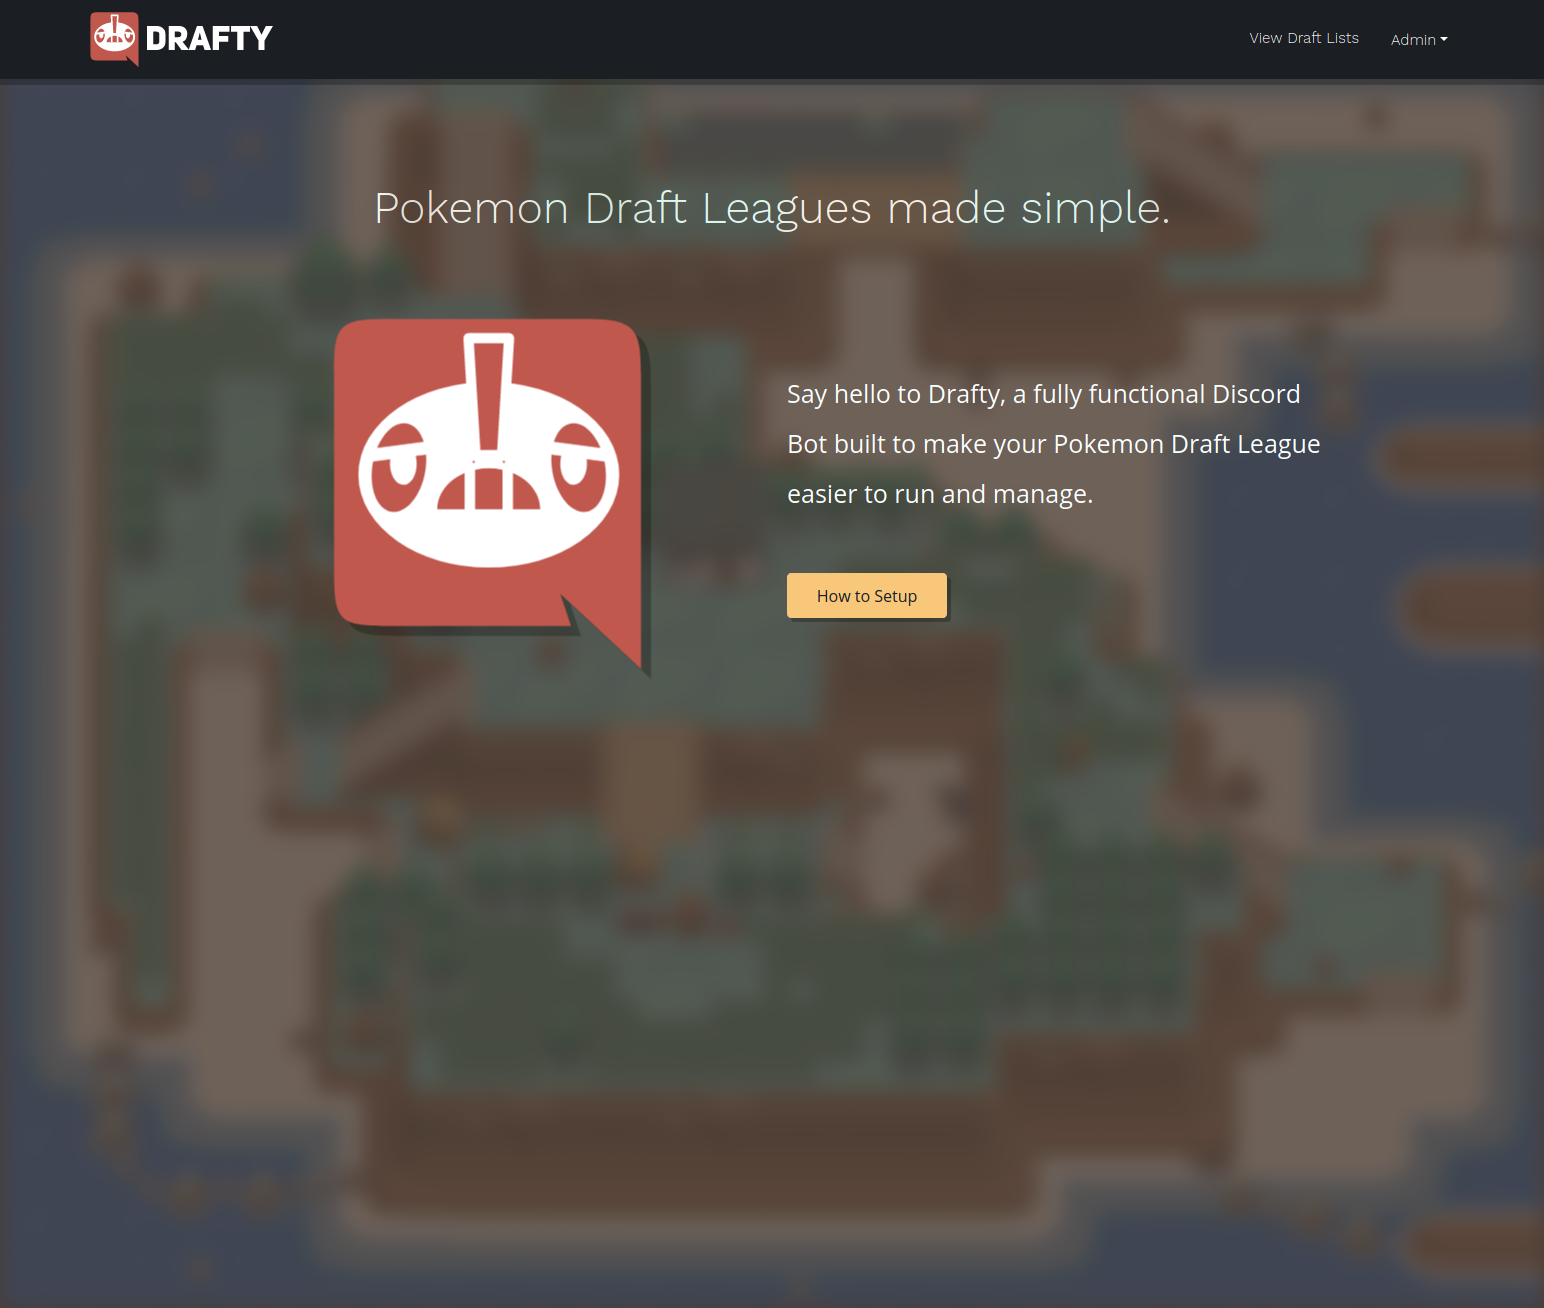
\includegraphics[scale=.3]{landing.png}

  \subsubsection*{Create League}
  To create a league,navigate to the Create League section under Admin on the navbar. Once there, the interface should be relatively straightforward. 
  First, give your leage a name, and decide on a format. Currently the only supported format Gen 8 OU. Next, Add users to the league. 
  Please note you cannot add users later, as the match schedule is determined upon creation of the league. 
  Each user can either be a coach or an admin, or both, but you CANNOT add a user that is neither. 
  An admin gets extra permissions in discord, such as the ability to turn drafting and redrafting on or off.
  Once all your users have been added, the next step is to select a tier list. 
  Currently, only premade lists are avaialble to use. But later on, the option to import your own will be supported.
  Last, hit the Submit League Button. Upon reload, your league will have been created!\\
  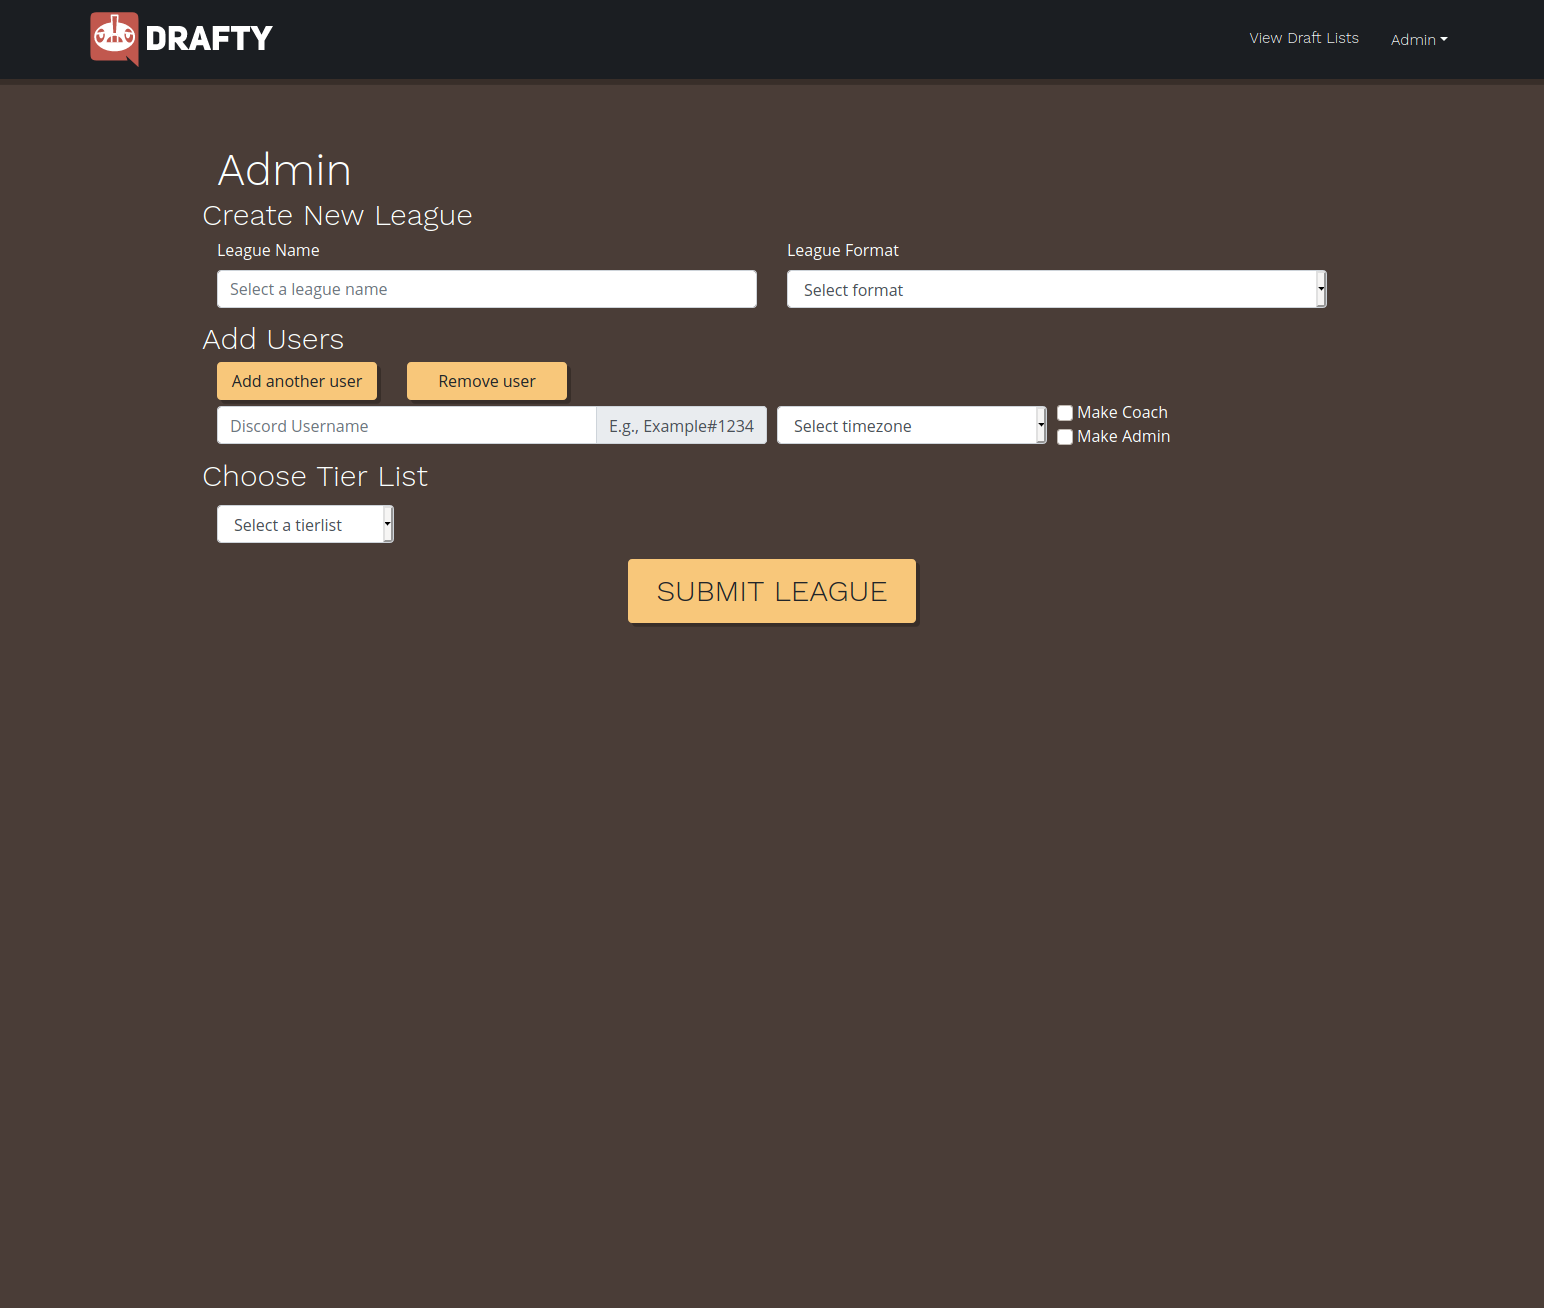
\includegraphics[scale=.3]{create_league.png}

  \subsubsection*{Manage League}
  To manage a league, navigate to the Manage League section under Admin on the navbar. Once there, you will have a couple options.
  You can either delete an entire league, or delete a user from a league. Deleting a league deletes all users, all teams, and all matches. 
  Deleting a user delete's that user's team and removes their matches.
  There will be Remove User section for each league, since each league has unique users. \\
  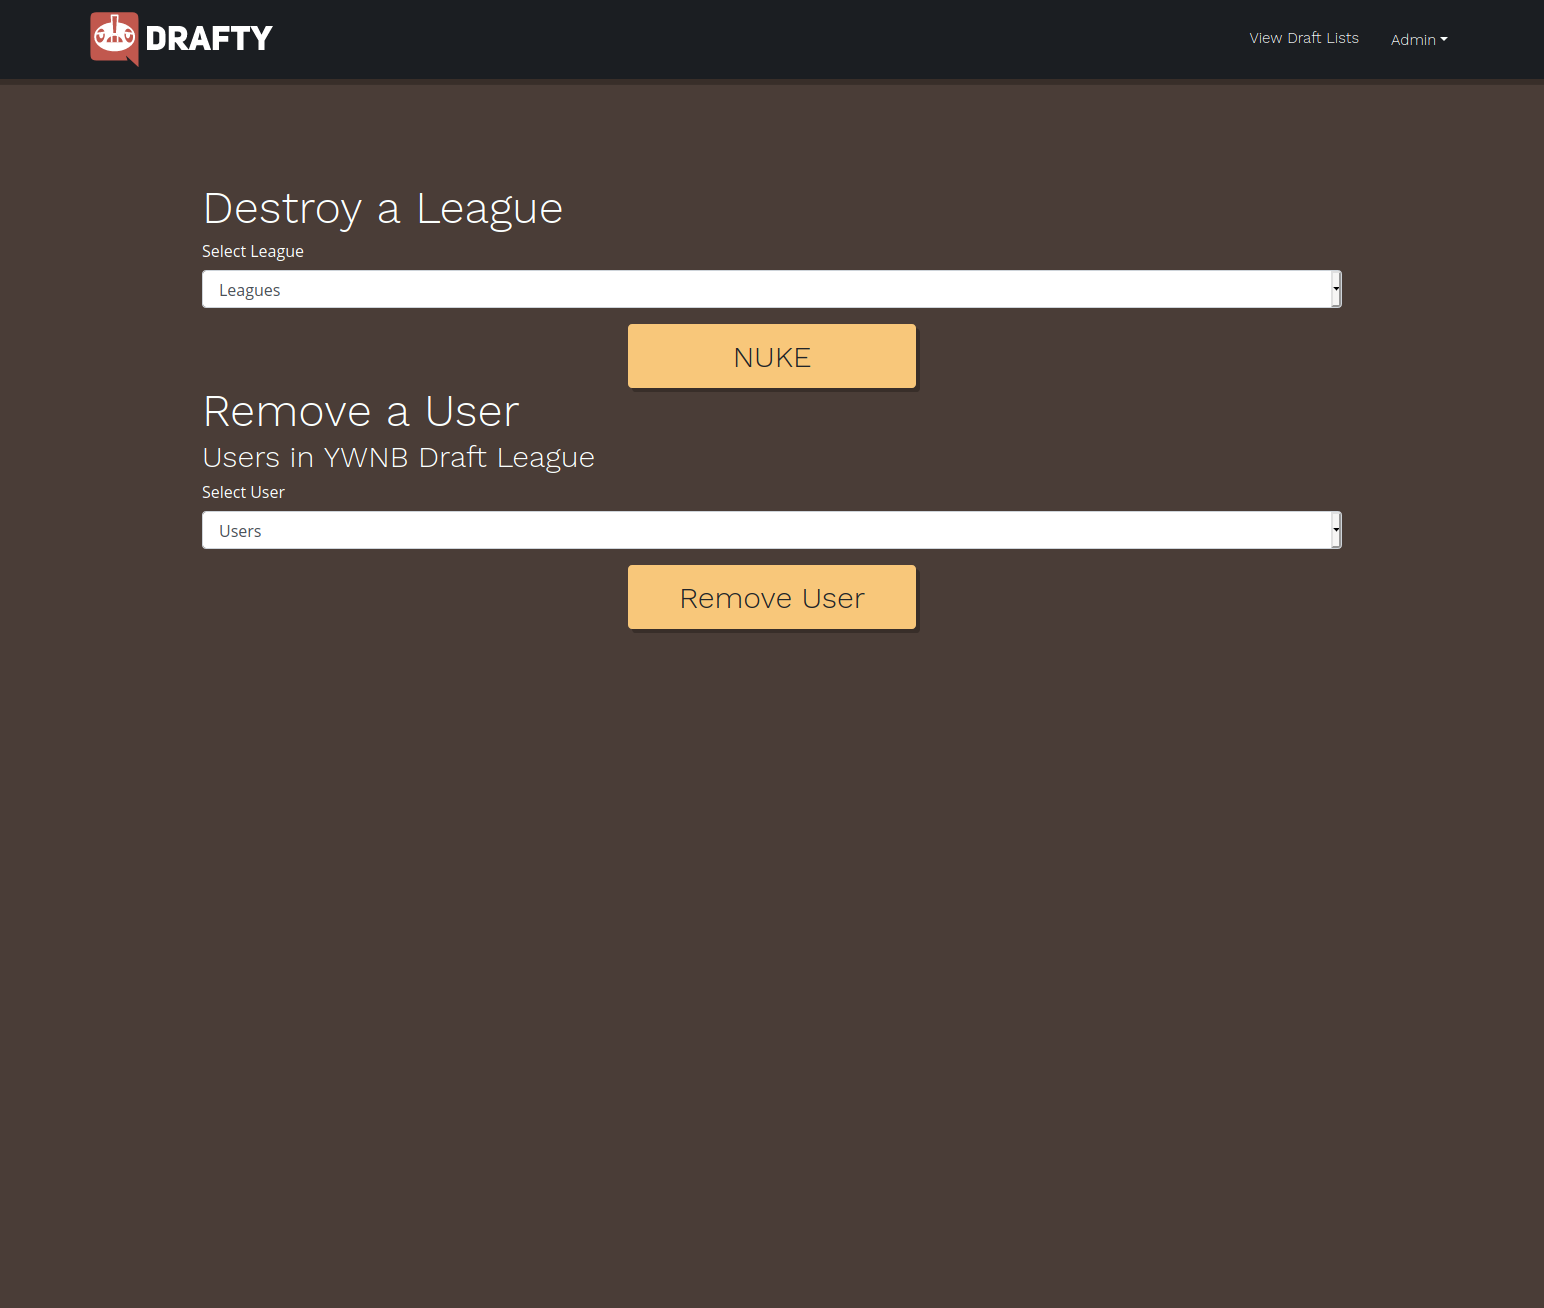
\includegraphics[scale=.3]{manage_league.png}

  \subsubsection*{View Draft List}
  To view a draft list, navigate to the View Draft Lists section. Once there, simply select a league and hit submit to view the draft list being used for that league.\\
  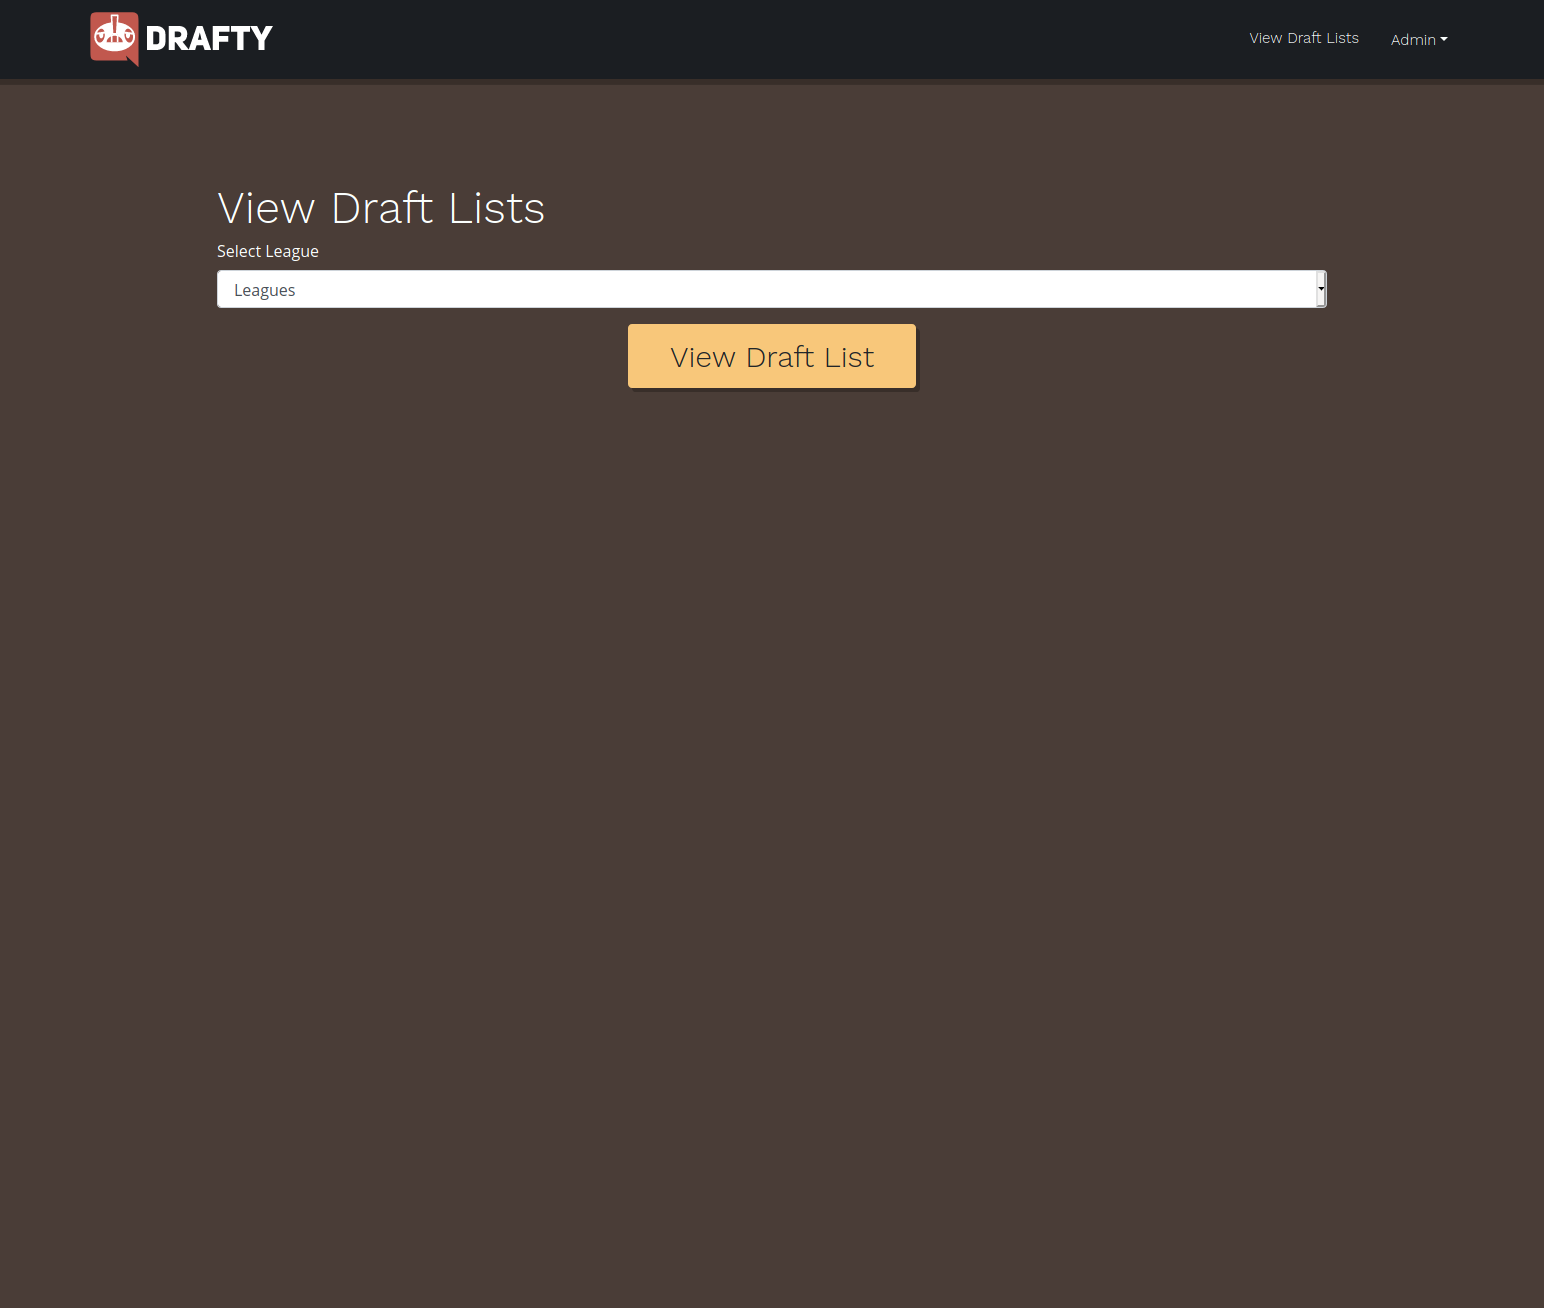
\includegraphics[scale=.3]{view_dl.png}
  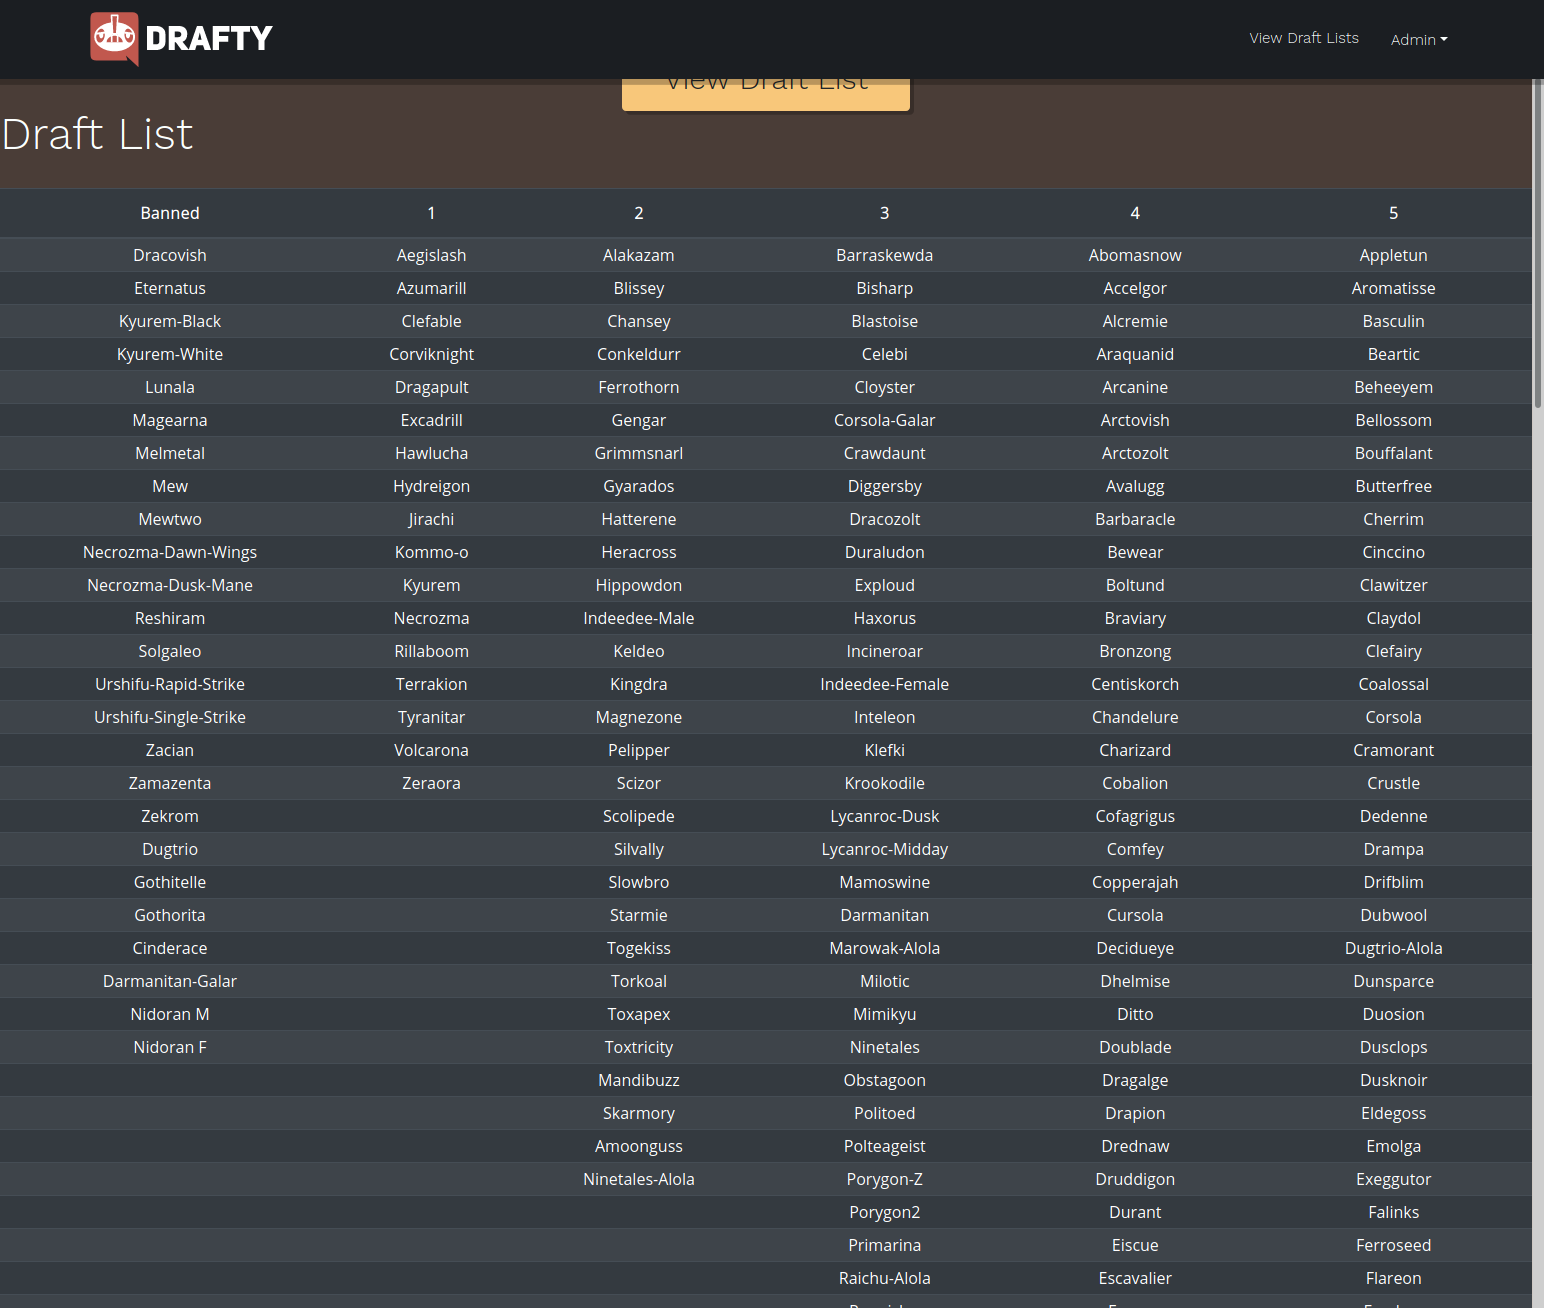
\includegraphics[scale=.3]{view_dl2.png}

\subsection*{Using The Discord Bot}
To start the Discord bot, run deploy\_bot.sh to begin the web application, and type in the name of the league you would like to run the league for. 
For more details, follow the instructions in Installation Instructions. 
The name of the league included in the dummy data is "YWNB Draft League"\\\\

\subsubsection*{Update showdown username}
The first step for all participants in the draft league is to register their showdown username. 
To do this, users should perform the following command: \verb|!regshowdown ohsnapplegcc|. 
Upon completion, if no one is already using that showdown username, Drafty will inform you that the update was a success.\\

\includegraphics[scale=.5]{regshowdown.png}
\\\\
\subsubsection*{Drafting}
To enable Pokemon drafting for teams, an admin must first enable it using \verb|!draft|. 
Once enabled, users are able to add Pokemon to their team.\\

\includegraphics[scale=.5]{draft.png}
\\\\
\subsubsection*{Redrafting}
To enable rerafting for teams, an admin must first enable it using \verb|!redraft|. 
Once enabled, users are able to swap out Pokemon in their team.\\

\includegraphics[scale=.5]{redraft.png}
\\\\
\subsubsection*{View Pokemon}
To quickly access a Pokemon's serebii page, simply enter \verb|!pokemon <pokemon name>|.\\
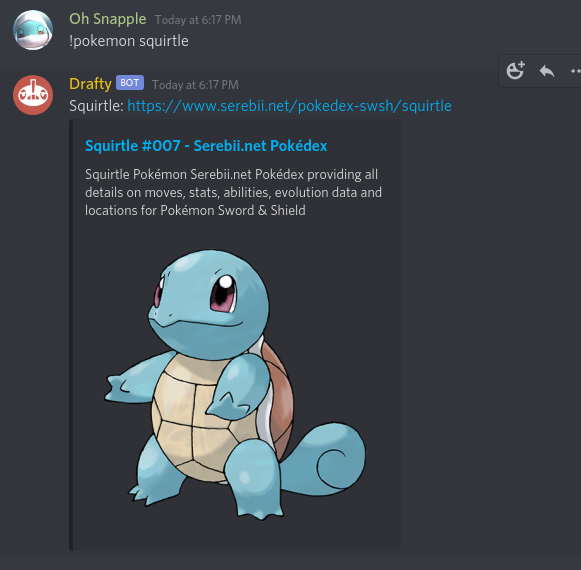
\includegraphics[scale=.5]{pokemon.png}
\\\\
\subsubsection*{View User Info}
To view a user's info, simply enter \verb|!userinfo <user's name>| to view all stats related to that coach and their team.
Alternatively, \verb|!userinfo| can be used with no parameters to view the userinfo for yourself.
When searching for a user, you can either type their full discord username (ex: Oh Snapple\#2136), or a piece of their name (ex: snapple).\\
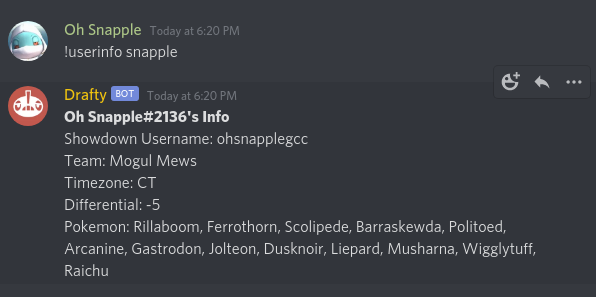
\includegraphics[scale=.5]{userinfo.png}
\\\\
\subsubsection*{Rankings}
To view the rankings in the league, type the commmand \verb|!rankings|. This will display the teams in order of differential.\\

\includegraphics[scale=.5]{rankings.png}
\\\\
\subsubsection*{Calculate Average Differential}
To view the average match differential for the league, type \verb|!average| or \verb|!avg|.\\
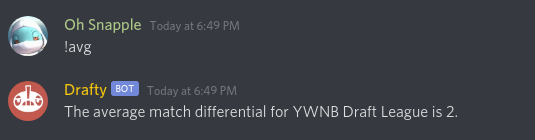
\includegraphics[scale=.5]{avg.png}
\\\\
\subsubsection*{View User's Matches}
To view all the matches a user plays in the league, type \verb|!matches <user's name>| or \verb|!matches|. 
This will display every match the user has to play in weekly order.\\
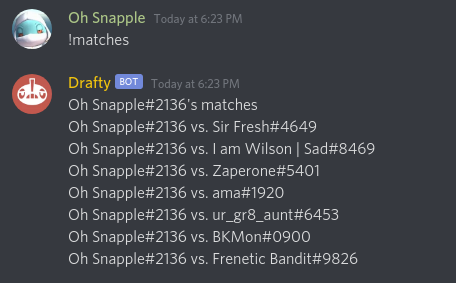
\includegraphics[scale=.5]{matches.png}
\\\\
\subsubsection*{View a Match Played}
To find the url for a specific match, type \verb|!match <user1>,<user2>|. \textbf{Make sure the usernames are seprated by a comma only.} 
This is because usernames can include spaces, so it is not a significant distiguisher. If a match hasn't been played, Drafty will let you know.\\
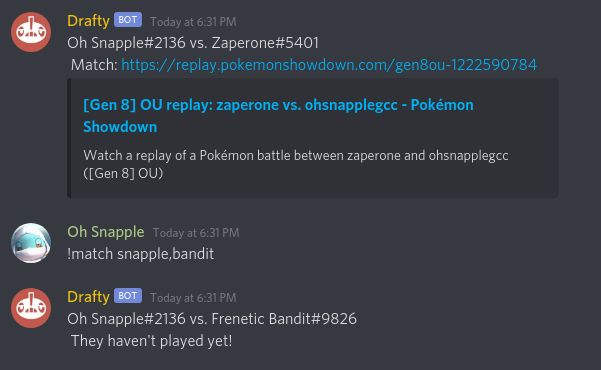
\includegraphics[scale=.5]{match_played.png}
\newpage
\subsubsection*{View User's Matches Played}
To get a list of all of a user's played matches, type \verb|!matchesplayed <username>|.
Alternatively, \verb|!matchesplayed|can be used to get urls for the matches played by the current discord user.\\ 
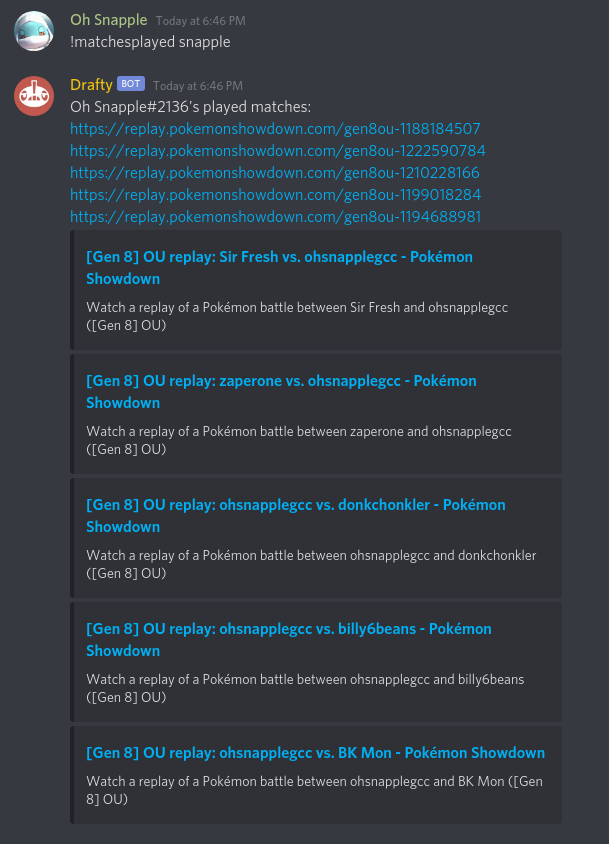
\includegraphics[scale=.5]{matches_played.png}
\newpage
\subsubsection*{Delete User}
Admins can delete users from the league through Drafty as well, simply type \verb|!delete <discord\_username>|.
The username must be exactly the user's discord name (ex: Oh Snapple\#2136). This is to ensure no accidental deletions.\\
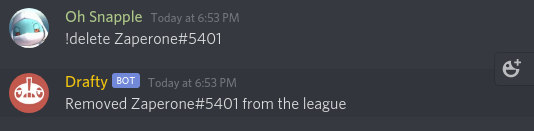
\includegraphics[scale=.5]{delete.png}


\end{document}
    